\documentclass[10pt]{book}
\usepackage[T1]{fontenc}
\usepackage[utf8]{inputenc}
\usepackage[italian]{babel}
\usepackage[document]{ragged2e}
%\usepackage{amsfonts}
%\usepackage{amssymb}
\usepackage{microtype}
%\usepackage{lmodern}
%\usepackage{fontspec}
%\usepackage{plex-serif} %
%\usepackage{plex-mono}
%\usepackage{stickstootext}
%\usepackage[usefilenames,DefaultFeatures={Ligatures=Common}]{plex-otf} %
%\usepackage[stickstoo,vvarbb]{newtxmath}
\usepackage{CharisSIL}
\usepackage[libertine]{newtxmath}
%\usepackage{erewhon}
%\usepackage{libertinus}
%\usepackage{inconsolata}
%\usepackage{notomath}
%\usepackage[bitstream-charter]{mathdesign}
%\usepackage[sfdefault]{AlegreyaSans}
%\usepackage[sfdefault,book]{FiraSans} %% option 'sfdefault' activates Fira Sans as the default text font
%\usepackage{FiraMono}
%\renewcommand*\oldstylenums[1]{{\firaoldstyle #1}}
\usepackage[all]{nowidow}
\usepackage{lettrine}
\usepackage{graphicx}
\usepackage{svg}
\usepackage[pdfa]{hyperref}
\usepackage{color}
\usepackage{setspace}
\usepackage{parskip}
\usepackage[Conny]{fncychap}
%\usepackage{fancyhdr}
%\pagestyle{fancy}
%\fancyhead[C,C]{\chaptermark}
%\fancyhead[R]{\textsc{Programmazione Avanzata}}
%\fancyfoot[R]{\thechapter}
%\fancyhead[LE,RO]{\textsc{\rightmark}}
%\fancyhead[LO,RE]{\textsc{\leftmark}}
%\fancyfoot[R]{\thepage}
%\renewcommand{\headrulewidth}{0.4pt}
%\renewcommand{\footrulewidth}{2pt}
%\renewcommand{\footrulewidth}{0.4pt}% default is 0pt
\usepackage[a4paper, inner=3.8cm, outer=4.7cm]{geometry}
\usepackage{listings}
\definecolor{dkgreen}{rgb}{0.1,0.5,0.1}
\definecolor{greengray}{rgb}{0.517,0.761,0.404}
\definecolor{orange}{rgb}{0.717,0.274,0.105}
\definecolor{blue}{rgb}{0.164,0.317,0.600}
\definecolor{background}{rgb}{0.990,0.990,0.990}
\lstset {
	frame=lrtb,
	language=java,
	aboveskip=0.7cm,
	belowskip=0.2cm,
	showstringspaces=false,
	columns=flexible,
	basicstyle={\small\ttfamily},
	numbers=none,
	backgroundcolor=\color{background},
	numberstyle=\tiny\color{dkgreen},
	keywordstyle=\color{blue},
	commentstyle=\color{greengray},
	stringstyle=\color{orange},
	breaklines=true,
	breakatwhitespace=true,
	tabsize=3
}

\newtheorem{thm}{Teorema}

\begin{document}
\setmonofont[Scale=.85]{Fira Code Retina}
\setstretch{1.25}

\title{Complessità}
\author{Marco Sgobino}
\maketitle
\tableofcontents

\part{Complessità}
\chapter{La macchina di Turing}
\section{Descrizione}

Una \emph{macchina di Turing} è una macchina che è descritta da un insieme di
\emph{simboli} $\Gamma = \{\alpha, \beta, \gamma, \delta, \dots\}$ finito e da
un insieme di \emph{stati} $\mathcal{Q} = \{q_1, q_2, \dots, q_n\}$ anch'esso
finito. La macchina di Turing dispone di un nastro di memoria potenzialmente
illimitato a destra e a sinistra; essa è in grado di identificare il simbolo
nella posizione dove la \emph{testina} della macchina è collocata sul nastro.
Ad ogni iterazione della macchina di Turing, viene letto il simbolo
ove sia collocata la sua testina; a seconda dello stato $q_i$, viene intrapresa
un'azione, che può essere una fra le $3$ seguenti:
\begin{itemize}
    \item spostamento della testina a destra;
    \item spostamento della testina a sinistra;
    \item riscrittura del simbolo sotto la testina con uno qualsiasi
        appartenente all'alfabeto di simboli.
\end{itemize}

Una macchina di Turing può anche essere accompagnato da un alfabeto
\emph{ausiliario}, ovverosia un alfabeto $\mathcal V$ comprendente simboli
simili a quelli di $\Gamma$, ma che vengono utilizzati qualora la macchina di
Turing avesse \emph{già processato} la cella in questione. Tipicamente,
l'utilizzo dell'alfabeto ausiliario è importante nel caso specifico in cui si
adoperino algoritmi e procedure per le quali è d'interesse ricordare se una
cella sia già stata in precedenza processata dalla macchina di Turing, oppure
no.

Nello specifico, una macchina di Turing è univocamente identificata dalla sua
\emph{matrice di transizione} $\delta  : \mathcal Q \times \Gamma \rightarrow
\mathcal Q \times (\Gamma \cup \{L,R\})$\footnote{In talune circostanze, è
possibile trovare una definizione differente, cioè $$\delta  : \mathcal Q \times
\Gamma \rightarrow \mathcal Q \times \Gamma \times \{L,R\};$$ in altre parole, è
una macchina che \emph{si muove sempre sul nastro,} poiché per ogni stato è
sempre definito un movimento. Per questo tipo di macchina, sono necessarie
diverse regole d'ingaggio, e i programmi in essa costruiti saranno radicalmente
differenti. La differenza fra i due modelli rappresenta un'evidenza della
versatilità della macchina di Turing.}, dove i simboli $L$ ed $R$ sono
rappresentativi dell'azione di spostarsi, rispettivamente, a sinistra e a
destra del nastro di memoria. La matrice di transizione lega, dunque, ciascuno
stato al simbolo collocato immediatamente sotto alla testina nel nastro di
memoria, stabilendo in maniera univoca l'azione da intraprendere. L'insieme
delle azioni che la macchina di Turing compie è quindi la realizzazione del
programma stesso.


\begin{table}[ht]
\centering
\begin{tabular}{c|cccc}
    & $q_1$ & $q_2$ & $\cdots$ & $q_n$ \\
    \hline
$\alpha$ & $\beta/q_2$ & $\gamma/q_2$ & $\cdots$ & \\
$\beta$ & $L/q_1$ & $\gamma/q_3$ & $\cdots$ & \\
$\gamma$ & $\gamma/q_3$ & $R/q_2$ & $\cdots$ & \\
$\vdots$ & $\vdots$ & $\vdots$ & $\ddots$ &    
\end{tabular}
\caption{Possibile matrice di transizione per una macchina di Turing. Le righe
corrispondono ai simboli dell'alfabeto $\Gamma$, mentre le colonne sono
corrispondenti ai singoli stati dell'insieme $\mathcal
Q$.}\label{tab:matriceTransizione}
\end{table}
\bigskip


Diversamente dal modello RAM, la quantità di memoria destinata ad ogni cella è
\emph{limitata}, poiché vi può essere collocato soltanto un numero finito di
simboli, quelli appunto dell'insieme $\Gamma$. Ciononostante, la macchina di
Turing si presta meglio alla trattazione di stringhe, poiché i simboli possono
rappresentare qualsivoglia tipologia di entità astratta, mentre per il modello
RAM si avrebbe necessità di una codifica fra numeri reali e simboli da
trattare: non vi è più dunque la limitazione imposta dal fatto che all'interno
di una cella possa risiedere esclusivamente un numero naturale, non importa
quanto grande sia; nella macchina di Turing le celle possono contenere simboli
di qualsiasi natura essi siano.

Tipicamente, all'alfabeto che definisce una macchina di Turing viene definito
un sottoinsieme sigma di simboli di input, $\Sigma \subset \Gamma$, in
concomitanza al quale viene definito un simbolo vuoto, \emph{blank}, $b \in
\Gamma - \Sigma$. Il simbolo $b$ rappresenta dunque l'idea di \emph{cella
vuota}. Ricapitolando, ogni macchina di Turing viene univocamente definita da:
\begin{itemize}
    \item un insieme finito di simboli $\Gamma$ \--- essi comprendono sia i
        simboli di input $\Sigma$ che il simbolo \emph{blank} $b$;
    \item un insieme finito di stati $\mathcal Q$;
    \item una funzione (matrice) di transizione $\delta  : \mathcal Q \times
        \Gamma \rightarrow \mathcal Q \times (\Gamma \cup \{L,R\})$.
\end{itemize}

Una diversa maniera per definire una macchina di Turing è tramite la
\emph{quaterna} o \emph{quadrupla} $q_i, s_j, \alpha, q_k$, dove $q_i$ è lo
\emph{stato in cui si trova la macchina}, $s_j$ è il \emph{simbolo letto dalla
testina}, $\alpha$ è il \emph{simbolo scritto nella matrice di transizione}, $q_k$ è
lo \emph{stato successivo} in cui la macchina di Turing si troverà al termine
dell'esecuzione di $\alpha$. In particolare, l'operazione che la macchina di
Turing effettua dipende dal simbolo $\alpha$ scritto nella matrice di
transizione:
\begin{itemize}
    \item se $\alpha = s_i$, sostituisci il simbolo $s_j$ con $s_i$;
    \item se $\alpha = R$, muovi la testina a destra;
    \item se $\alpha = L$, muovi la testina a sinistra;
\end{itemize}

Lo \emph{stop} della computazione di una macchina di Turing avviene qualora la
coppia $q_i, s_j$ \textbf{non} sia presente nella matrice di transizione. In
tal caso, la macchina di Turing si fermerà, e vi sarà il riconoscimento del
valore finale di computazione, espresso come nel caso del modello RAM con una
convenzione che permetta di identificare il valore finale del risultato della
computazione.

\section{Uso di una macchina di Turing}

Una macchina di Turing, come verrà illustrato in seguito, può essere espressa
anche mediante \emph{grafo} oltre che mediante matrice di sostituzione. In ogni
caso, tutte le possibili definizioni di macchina di Turing sono del tutto
equivalenti, e variano esclusivamente nella forma nella quale esse sono
proposte. Una macchina di Turing, non importa come sia stata definita, può
essere adoperata sostanzialmente per $3$ diversi compiti:
\begin{enumerate}
    \item per il \emph{calcolo} di una funzione \--- la macchina di Turing è
        intesa come \emph{calcolatore}, e lo scopo è quello di calcolare una
        funzione $f: \mathbb{N}^n \rightarrow \mathbb{N}$. In questo caso, la
        macchina di Turing risulta essere meno efficiente del modello RAM, per
        via dell'assenza del comodo sistema di istruzioni presente in quest
        ultimo;
    \item per il \emph{riconoscimento} di una stringa \--- la macchina di
        Turing è intesa come \emph{accettore}. In questo contesto la MdT è
        molto più efficiente del modello RAM, poiché non è richiesta la
        codifica da numeri naturali a simboli;
    \item per la \emph{decisione} di un predicato \--- la macchina di Turing è
        intesa come \emph{decisore}.
\end{enumerate}

TODO aggiungi esito macchina di turing
TODO aggiungi esito vettoriale mdt

Solitamente, è particolarmente difficile programmare sulla macchina di
Turing~\--~questo è principalmente dovuto al fatto che la macchina di Turing è
una macchina a stati, dove non vi è un insieme di istruzioni da applicare
direttamente, ma bisogna determinare la matrice di transizione relativa a ciò
che bisogna calcolare, stato per stato e simbolo per simbolo.


\section{Equivalenza fra macchina di Turing e $\mathcal R$}

Un importante teorema definisce l'equivalenza della macchina di Turing (avente
insieme delle funzioni computabili $\mathcal{TC}$ all'insieme delle funzioni
parziali ricorsive $\mathcal R$, e lo lega indissolubilmente all'insieme delle
funzioni computabili dal modello RAM $\mathcal C$.

\begin{thm}{dell'equivalenza della macchina di Turing all'insieme $\mathcal R$}
    $$\mathcal R \equiv \mathcal {TC} \equiv \mathcal C$$
\end{thm}

Un possibile spunto di dimostrazione di $\mathcal {TC} \subseteq \mathcal R$ si
ha per il fatto che la configurazione e lo stato della MdT durante la
computazione possono essere codificati da un numero naturale; le operazioni
sulla macchina sono rappresentate da funzioni ricorsive su questi numeri. Il
viceversa è invece mostrabile tenendo conto che si può verificare che
$\mathcal{TC}$ contiene le funzioni di base ed è chiusa rispetto a sostituzione,
ricorsione e minimazione illimitata.

\section{Potenziamento apparente della macchina di Turing}

Una macchina di Turing può essere potenziata mediante l'estensione di essa
tramite l'uso di \emph{nastri multitraccia}. In altre parole, anziché adoperare
un singolo nastro, si adoperano più nastri contemporaneamente. La macchina di
Turing viene espansa tramite l'aggiunta di uno \emph{stato della memoria
suppletiva}, che sostanzialmente ci indica il numero del nastro dove la
macchina di Turing sta agendo. Dunque, ci possiamo immaginare una macchina di
Turing con tanti nastri e tante testine che lavorano contemporaneamente, come
elencato in Figura~\ref{fig:macchina-turing-multinastro}.

\begin{figure}[b]
    \centering
    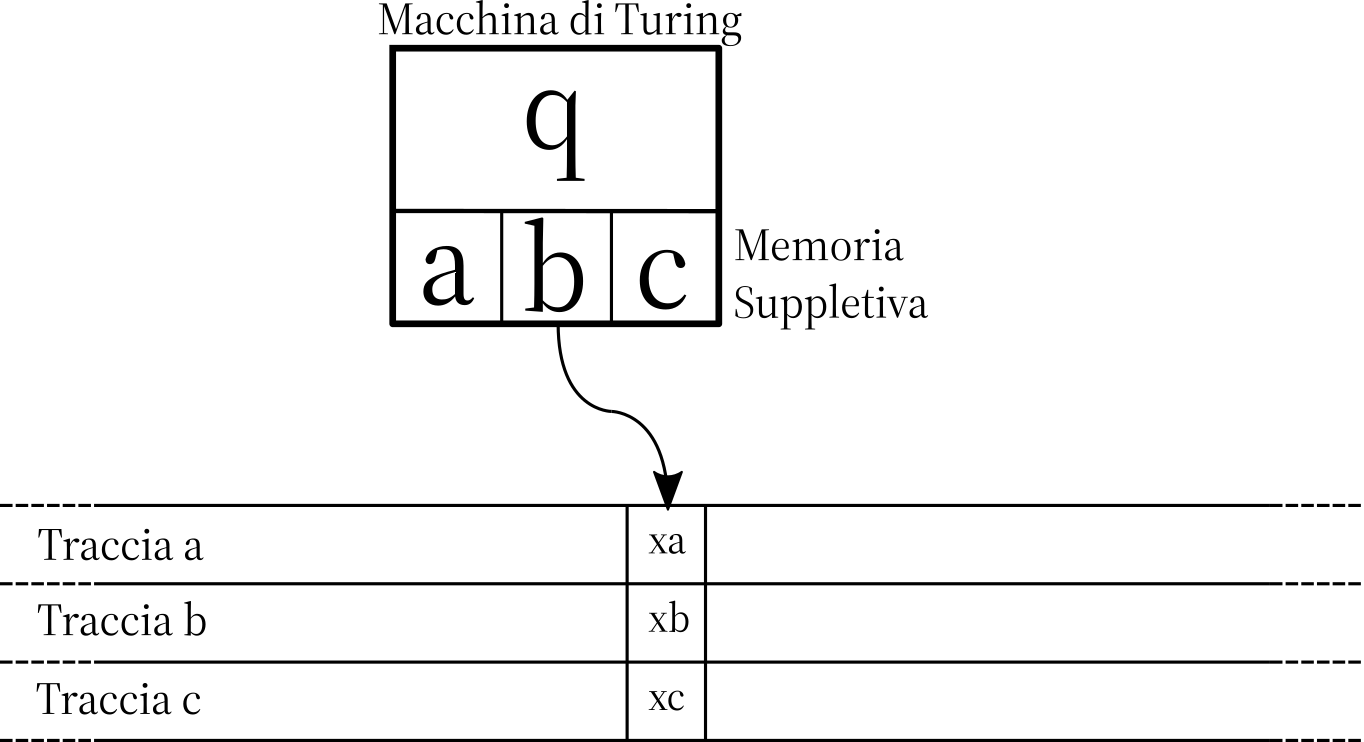
\includegraphics[ width=.8\linewidth, height=\textheight, keepaspectratio]{./pics/macchina-turing-multinastro.png}
    \caption{Macchina con memoria con nastro multitraccia.}
    \label{fig:macchina-turing-multinastro}
\end{figure}

Dal punto di vista della capacità computazione, una macchina di Turing
multinastro non aumenta né diminuisce le capacità \-- tuttavia, tale
rappresentazione può prestare una maggiore somiglianza con il tipo di
computazione svolto all'interno di un computer moderno. Si pensi infatti alla memoria
RAM, alla memoria cache, al disco rigido e così via; una macchina di Turing può
dunque ``simulare'' qualsiasi computer moderno\footnote{Un computer può a sua
volta simulare da una macchina di Turing, dal momento che possono essere
applicati potenzialmente infiniti banchi di memoria al computer \-- nella
pratica, tuttavia, sappiamo che ciò non è possibile, e i banchi di memoria non
saranno mai del tutto \emph{illmitati}}. Una macchina di Turing multinastro
deve essere implementata con un \emph{sistema multitraccia} \-- in altre
parole, vengono adoperate \emph{tante testine quante sono i nastri}. Ci si può
facilmente ricondurre alla macchina di Turing convenzionale semplicemente
eliminando il sistema multitraccia, o per meglio dire, una macchina di Turing
multitraccia può essere \emph{simulata} da una macchina di Turing
convenzionale: essa dunque, non produce alcun tipo di miglioramento dal punto
di vista computazione, cioè le due macchine hanno la \emph{stessa} potenza
computazionale (Figura~\ref{fig:mdt-equivalenza-multitraccia}. Il medesimo
discorso si applica anche tentando di \emph{menomare} la macchina di Turing,
nel senso che potremmo pensare di rendere il nastro semi-infinito, cioè
illimitato solo a destra o solo a sinistra
(Figura~\ref{fig:macchina-turing-riduzione}).
\begin{figure}[b]
    \centering
    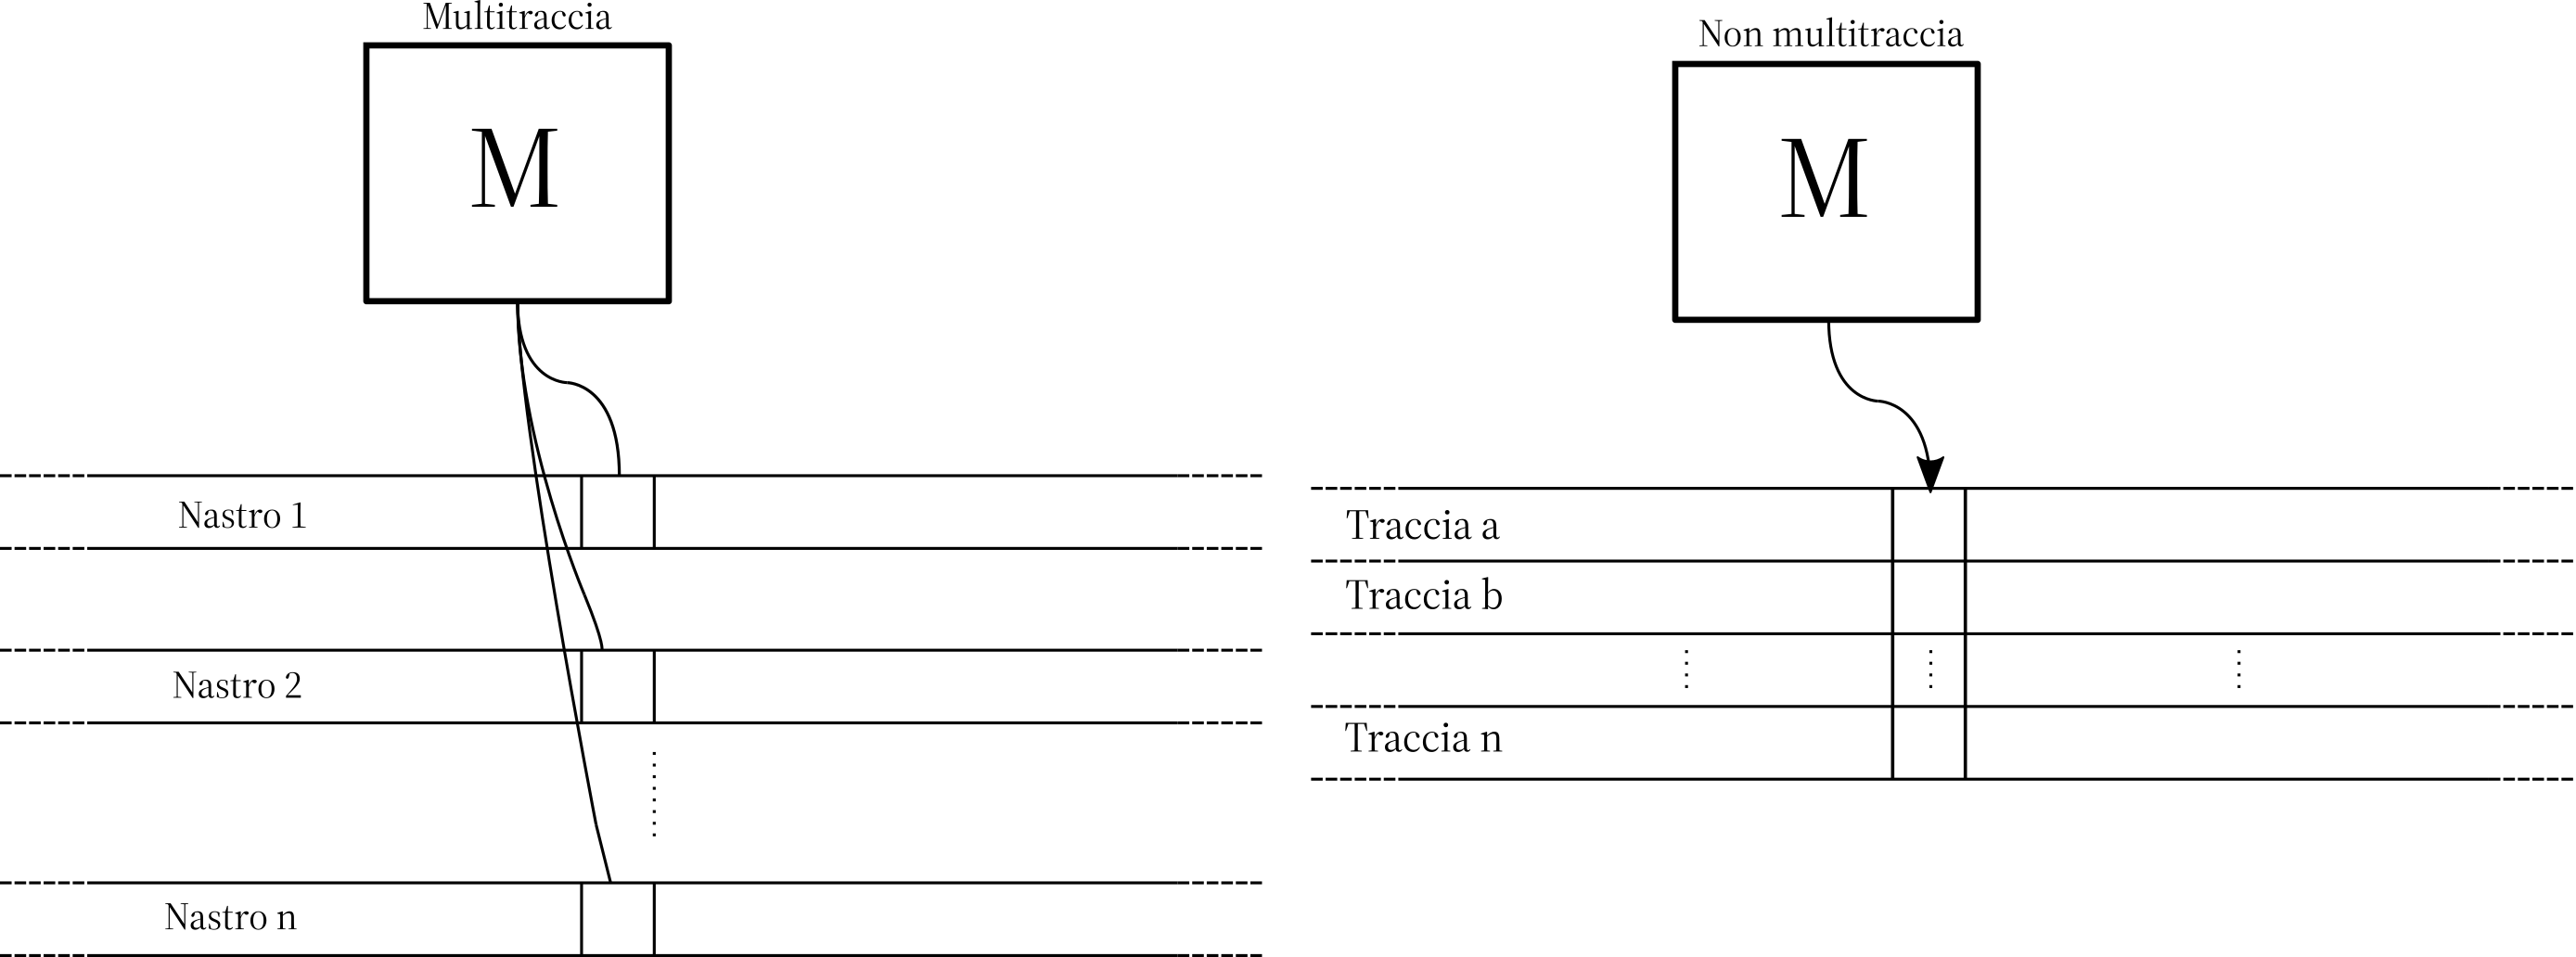
\includegraphics[ width=.7\linewidth, height=\textheight, keepaspectratio]{./pics/mdt-equivalenza-multitraccia.png}
    \caption{Equivalenza fra una macchina di Turing a multitraccia e una
    macchina di Turing a singola testina.}
    \label{fig:mdt-equivalenza-multitraccia}
\end{figure}

\begin{figure}[b]
    \centering
    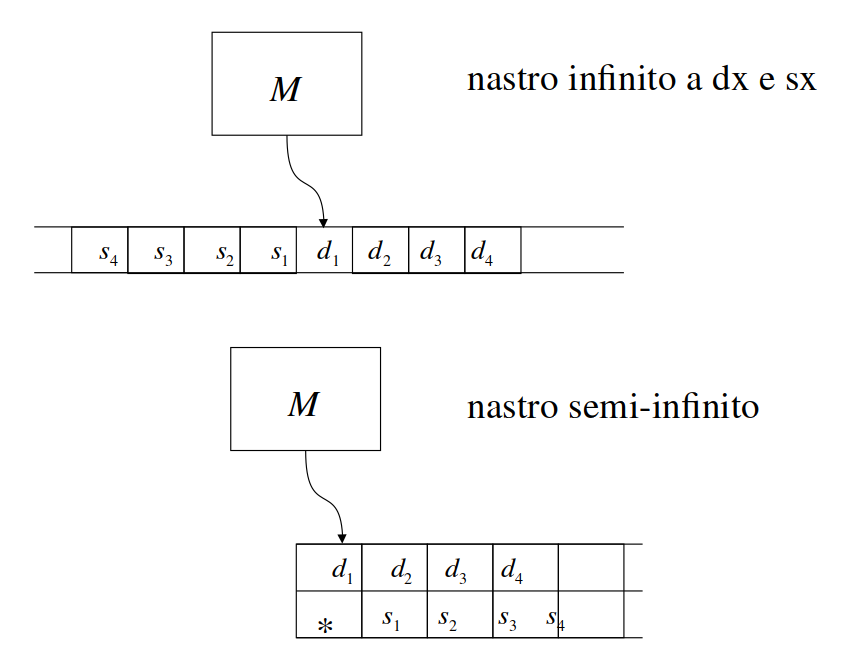
\includegraphics[ width=.7\linewidth, height=\textheight, keepaspectratio]{./pics/macchina-turing-riduzione.png}
    \caption{Equivalenza fra macchina di Turing a nastro illimitato solo a
    destra e a nastro illimitato da ambedue le parti.}
    \label{fig:macchina-turing-riduzione}
\end{figure}

\clearpage


\section{Macchina RAM per \emph{accettare} stringhe}

Nel modello RAM, per accettare una stringa è necessario operare una codifica.
In particolare, la stringa viene codificata in un numero naturale e la macchina
risponde con ``1'' o ``0'' a seconda che la stringa venga o meno accettata. Con
la macchina di Turing, invece, si può far intervenire direttamente uno
\emph{stato di accettazione} $q_Y$ o uno \emph{stato di rifiuto} $q_N$.
Un'altra possibilità è quella di semi-decidere riguardo l'accettazione di una
stringa, cioè una macchina in grado di riconoscere la stringa in questione, ma
di non poter rifiutare la stringa, poiché ci sarebbe un'infinita computazione,
e dunque divergenza. Tipicamente, lo stato iniziale viene denotato con $q_0$, e
potrebbero esserci degli stati ulteriori ``intermedi''. Un esempio di
accettazione è dato dalla macchina illustrata in
Figura~\ref{fig:mdtAccettazione1}. La macchina riconosce il linguaggio dato
dalle stringhe con due ``zeri'' nelle ultime due posizioni a destra, in
particolare tutte le stringhe che terminano con ``00''.

\begin{figure}[b]
    \centering
    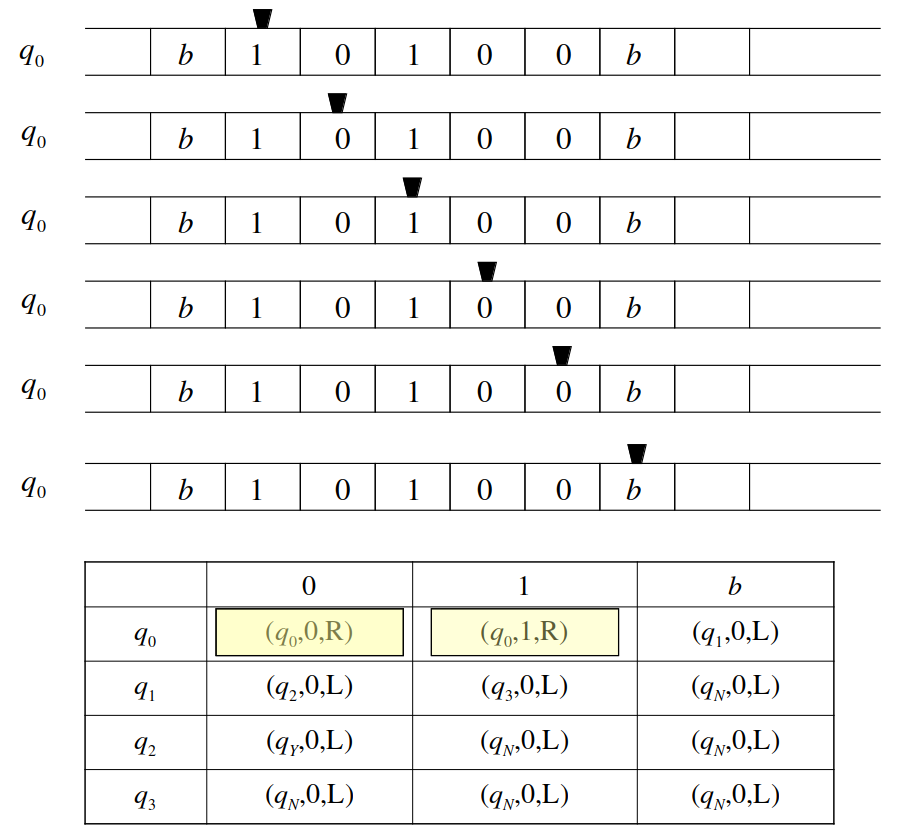
\includegraphics[ width=1.0\linewidth, height=\textheight, keepaspectratio]{./pics/mdtAccettazione1.png}
    \caption{Macchina che riconosce il linguaggio dato dalle stringhe con due $0$
nelle ultime due posizioni a destra, e suo funzionamento.}
    \label{fig:mdtAccettazione1}
\end{figure}

TODO aggiungi mdt definita a grafo

Una macchina di Turing può anche essere ``definita a grafo''. In questo modello
di definizione, la macchina di Turing,
\begin{itemize}
    \item ha un \emph{nastro semi-illimitato} a destra, diviso in celle;
    \item ha un alfabeto \emph{ausiliario} $\mathcal V$;
    \item ha un simbolo di spaziatura $\Delta$, equivalente al simbolo
        \emph{blank} $b$;
    \item un puntatore, del tutto equivalente alla testina;
    \item un \emph{programma}, definito come \textbf{grafo finito orientato},
        con i vertici definiti come \emph{stato}. Vi è uno stato di inizio,
        indicato con \textsc{Inizio}, e un sottoinsieme eventualmente vuoto di
        stati di arresto, indicati con \textsc{Accettazione}. I nodi del grafo
        sono collegati da \emph{archi}.
\end{itemize}

Ciascun arco è della forma

\begin{verbatim}
(i) ---(alpha, beta, gamma) ---> (j)
\end{verbatim}

dove $$\alpha \in \Sigma \cup \mathcal V \cup \{\Delta\}, \beta \in \Sigma \cup
\mathcal V \cup \{\Delta\} \mbox{ e } \gamma \in \{L, R\}.$$ Dunque, siamo
nello stato $i$; la macchina legge $\alpha$, scrive $\beta$ al posto di
$\alpha$, e infine va a destra oppure a sinistra a seconda che il simbolo
$\gamma$ sia pari ad $R$ o ad $L$.







\end{document}
